\documentclass[]{article}
\usepackage{lmodern}
\usepackage{amssymb,amsmath}
\usepackage{ifxetex,ifluatex}
\usepackage{fixltx2e} % provides \textsubscript
\ifnum 0\ifxetex 1\fi\ifluatex 1\fi=0 % if pdftex
  \usepackage[T1]{fontenc}
  \usepackage[utf8]{inputenc}
\else % if luatex or xelatex
  \ifxetex
    \usepackage{mathspec}
  \else
    \usepackage{fontspec}
  \fi
  \defaultfontfeatures{Ligatures=TeX,Scale=MatchLowercase}
\fi
% use upquote if available, for straight quotes in verbatim environments
\IfFileExists{upquote.sty}{\usepackage{upquote}}{}
% use microtype if available
\IfFileExists{microtype.sty}{%
\usepackage{microtype}
\UseMicrotypeSet[protrusion]{basicmath} % disable protrusion for tt fonts
}{}
\usepackage[margin=1in]{geometry}
\usepackage{hyperref}
\hypersetup{unicode=true,
            pdftitle={Final Report},
            pdfauthor={Carleena Ortega and Saelin Bjornson},
            pdfborder={0 0 0},
            breaklinks=true}
\urlstyle{same}  % don't use monospace font for urls
\usepackage{longtable,booktabs}
\usepackage{graphicx,grffile}
\makeatletter
\def\maxwidth{\ifdim\Gin@nat@width>\linewidth\linewidth\else\Gin@nat@width\fi}
\def\maxheight{\ifdim\Gin@nat@height>\textheight\textheight\else\Gin@nat@height\fi}
\makeatother
% Scale images if necessary, so that they will not overflow the page
% margins by default, and it is still possible to overwrite the defaults
% using explicit options in \includegraphics[width, height, ...]{}
\setkeys{Gin}{width=\maxwidth,height=\maxheight,keepaspectratio}
\IfFileExists{parskip.sty}{%
\usepackage{parskip}
}{% else
\setlength{\parindent}{0pt}
\setlength{\parskip}{6pt plus 2pt minus 1pt}
}
\setlength{\emergencystretch}{3em}  % prevent overfull lines
\providecommand{\tightlist}{%
  \setlength{\itemsep}{0pt}\setlength{\parskip}{0pt}}
\setcounter{secnumdepth}{0}
% Redefines (sub)paragraphs to behave more like sections
\ifx\paragraph\undefined\else
\let\oldparagraph\paragraph
\renewcommand{\paragraph}[1]{\oldparagraph{#1}\mbox{}}
\fi
\ifx\subparagraph\undefined\else
\let\oldsubparagraph\subparagraph
\renewcommand{\subparagraph}[1]{\oldsubparagraph{#1}\mbox{}}
\fi

%%% Use protect on footnotes to avoid problems with footnotes in titles
\let\rmarkdownfootnote\footnote%
\def\footnote{\protect\rmarkdownfootnote}

%%% Change title format to be more compact
\usepackage{titling}

% Create subtitle command for use in maketitle
\providecommand{\subtitle}[1]{
  \posttitle{
    \begin{center}\large#1\end{center}
    }
}

\setlength{\droptitle}{-2em}

  \title{Final Report}
    \pretitle{\vspace{\droptitle}\centering\huge}
  \posttitle{\par}
    \author{Carleena Ortega and Saelin Bjornson}
    \preauthor{\centering\large\emph}
  \postauthor{\par}
      \predate{\centering\large\emph}
  \postdate{\par}
    \date{15/03/2020}


\begin{document}
\maketitle

{
\setcounter{tocdepth}{4}
\tableofcontents
}
\hypertarget{adult-income}{%
\subsection{Adult Income}\label{adult-income}}

\hypertarget{introduction}{%
\subsubsection{Introduction}\label{introduction}}

\hypertarget{the-dataset}{%
\paragraph{The Dataset}\label{the-dataset}}

Who: The data set was extracted by Barry Becker from the 1994 Census
database and is donated by Silicon Graphics\\
What: This is a multivariate dataset with categorical and integer
variables. It contains the predicted income of individuals from the
census with attributes including age, marital status, work class,
education, sex, and race.\\
When: The data is from a 1994 census.\\
Why: The data set is found in the University of California Irvine
Machine Learning Repository, and was used for ML prediction of whether a
person makes over or under 50K a year based on their attributes.\\
How: The census data was collected by survey.

\hypertarget{the-variables}{%
\paragraph{The Variables}\label{the-variables}}

\begin{longtable}[]{@{}lll@{}}
\toprule
\begin{minipage}[b]{0.35\columnwidth}\raggedright
Variable\strut
\end{minipage} & \begin{minipage}[b]{0.30\columnwidth}\raggedright
Type\strut
\end{minipage} & \begin{minipage}[b]{0.26\columnwidth}\raggedright
Description\strut
\end{minipage}\tabularnewline
\midrule
\endhead
\begin{minipage}[t]{0.35\columnwidth}\raggedright
age\strut
\end{minipage} & \begin{minipage}[t]{0.30\columnwidth}\raggedright
int\strut
\end{minipage} & \begin{minipage}[t]{0.26\columnwidth}\raggedright
Age of individual\strut
\end{minipage}\tabularnewline
\begin{minipage}[t]{0.35\columnwidth}\raggedright
workclass\strut
\end{minipage} & \begin{minipage}[t]{0.30\columnwidth}\raggedright
chr\strut
\end{minipage} & \begin{minipage}[t]{0.26\columnwidth}\raggedright
e.g.~private, self-emplowed, federal government, never worked,
etc.\strut
\end{minipage}\tabularnewline
\begin{minipage}[t]{0.35\columnwidth}\raggedright
fnlwgt\strut
\end{minipage} & \begin{minipage}[t]{0.30\columnwidth}\raggedright
int\strut
\end{minipage} & \begin{minipage}[t]{0.26\columnwidth}\raggedright
Final weights: weighted sums of the socio-economic characteristics of
the individual. People with similar demographics have similar
weights.\strut
\end{minipage}\tabularnewline
\begin{minipage}[t]{0.35\columnwidth}\raggedright
education\strut
\end{minipage} & \begin{minipage}[t]{0.30\columnwidth}\raggedright
chr\strut
\end{minipage} & \begin{minipage}[t]{0.26\columnwidth}\raggedright
Highest education recieved\strut
\end{minipage}\tabularnewline
\begin{minipage}[t]{0.35\columnwidth}\raggedright
educationnum\strut
\end{minipage} & \begin{minipage}[t]{0.30\columnwidth}\raggedright
factor\strut
\end{minipage} & \begin{minipage}[t]{0.26\columnwidth}\raggedright
Numerical code for highest education recieved\strut
\end{minipage}\tabularnewline
\begin{minipage}[t]{0.35\columnwidth}\raggedright
marital\_status\strut
\end{minipage} & \begin{minipage}[t]{0.30\columnwidth}\raggedright
int\strut
\end{minipage} & \begin{minipage}[t]{0.26\columnwidth}\raggedright
e.g.~married, never married, divorced, etc.\strut
\end{minipage}\tabularnewline
\begin{minipage}[t]{0.35\columnwidth}\raggedright
occupation\strut
\end{minipage} & \begin{minipage}[t]{0.30\columnwidth}\raggedright
chr\strut
\end{minipage} & \begin{minipage}[t]{0.26\columnwidth}\raggedright
Occupation of individual\strut
\end{minipage}\tabularnewline
\begin{minipage}[t]{0.35\columnwidth}\raggedright
relationship\strut
\end{minipage} & \begin{minipage}[t]{0.30\columnwidth}\raggedright
chr\strut
\end{minipage} & \begin{minipage}[t]{0.26\columnwidth}\raggedright
Relation of individual in family. e.g.~wife, child, husband,
unmarried\strut
\end{minipage}\tabularnewline
\begin{minipage}[t]{0.35\columnwidth}\raggedright
race\strut
\end{minipage} & \begin{minipage}[t]{0.30\columnwidth}\raggedright
chr\strut
\end{minipage} & \begin{minipage}[t]{0.26\columnwidth}\raggedright
Asian-Pacific Islander, Native American, White, Black, other\strut
\end{minipage}\tabularnewline
\begin{minipage}[t]{0.35\columnwidth}\raggedright
sex\strut
\end{minipage} & \begin{minipage}[t]{0.30\columnwidth}\raggedright
chr\strut
\end{minipage} & \begin{minipage}[t]{0.26\columnwidth}\raggedright
Male or Female\strut
\end{minipage}\tabularnewline
\begin{minipage}[t]{0.35\columnwidth}\raggedright
capital\_gain\strut
\end{minipage} & \begin{minipage}[t]{0.30\columnwidth}\raggedright
int\strut
\end{minipage} & \begin{minipage}[t]{0.26\columnwidth}\raggedright
Profit from capital assets such as investments, real estate, etc.\strut
\end{minipage}\tabularnewline
\begin{minipage}[t]{0.35\columnwidth}\raggedright
capital\_loss\strut
\end{minipage} & \begin{minipage}[t]{0.30\columnwidth}\raggedright
int\strut
\end{minipage} & \begin{minipage}[t]{0.26\columnwidth}\raggedright
Loss from capital assets\strut
\end{minipage}\tabularnewline
\begin{minipage}[t]{0.35\columnwidth}\raggedright
hours\_per\_week\strut
\end{minipage} & \begin{minipage}[t]{0.30\columnwidth}\raggedright
\strut
\end{minipage} & \begin{minipage}[t]{0.26\columnwidth}\raggedright
The number of hours that the individual works per week\strut
\end{minipage}\tabularnewline
\begin{minipage}[t]{0.35\columnwidth}\raggedright
country\strut
\end{minipage} & \begin{minipage}[t]{0.30\columnwidth}\raggedright
chr\strut
\end{minipage} & \begin{minipage}[t]{0.26\columnwidth}\raggedright
Country of origin\strut
\end{minipage}\tabularnewline
\begin{minipage}[t]{0.35\columnwidth}\raggedright
income\strut
\end{minipage} & \begin{minipage}[t]{0.30\columnwidth}\raggedright
chr\strut
\end{minipage} & \begin{minipage}[t]{0.26\columnwidth}\raggedright
Whether individual is predicted to make over or under 50K\strut
\end{minipage}\tabularnewline
\bottomrule
\end{longtable}

mentioned the renamed/ grouped factors here

\hypertarget{the-research-questions}{%
\paragraph{The Research Questions}\label{the-research-questions}}

\begin{enumerate}
\def\labelenumi{\arabic{enumi}.}
\tightlist
\item
  Is hours worked per week correlated with age, relationship, education
  level, or sex?
\end{enumerate}

Plots showing the relationship between hours worked and each variable
separately. For example, we will use the linear regression model to
explore how hours at work is related to variables such as age,
relationship, education level, and sex.

\hypertarget{exploratory-data-analysis}{%
\subsubsection{Exploratory Data
Analysis}\label{exploratory-data-analysis}}

In this section, we will get to know our dataset better by exploring the
relationship between certain factors.

\hypertarget{age-and-sex}{%
\paragraph{Age and Sex}\label{age-and-sex}}

The plot below shows that there are more male employees than female
employees and that the majority of working males are older than working
females since the male (blue curve) have a peak shifted to the right
with respect to female (red peak).

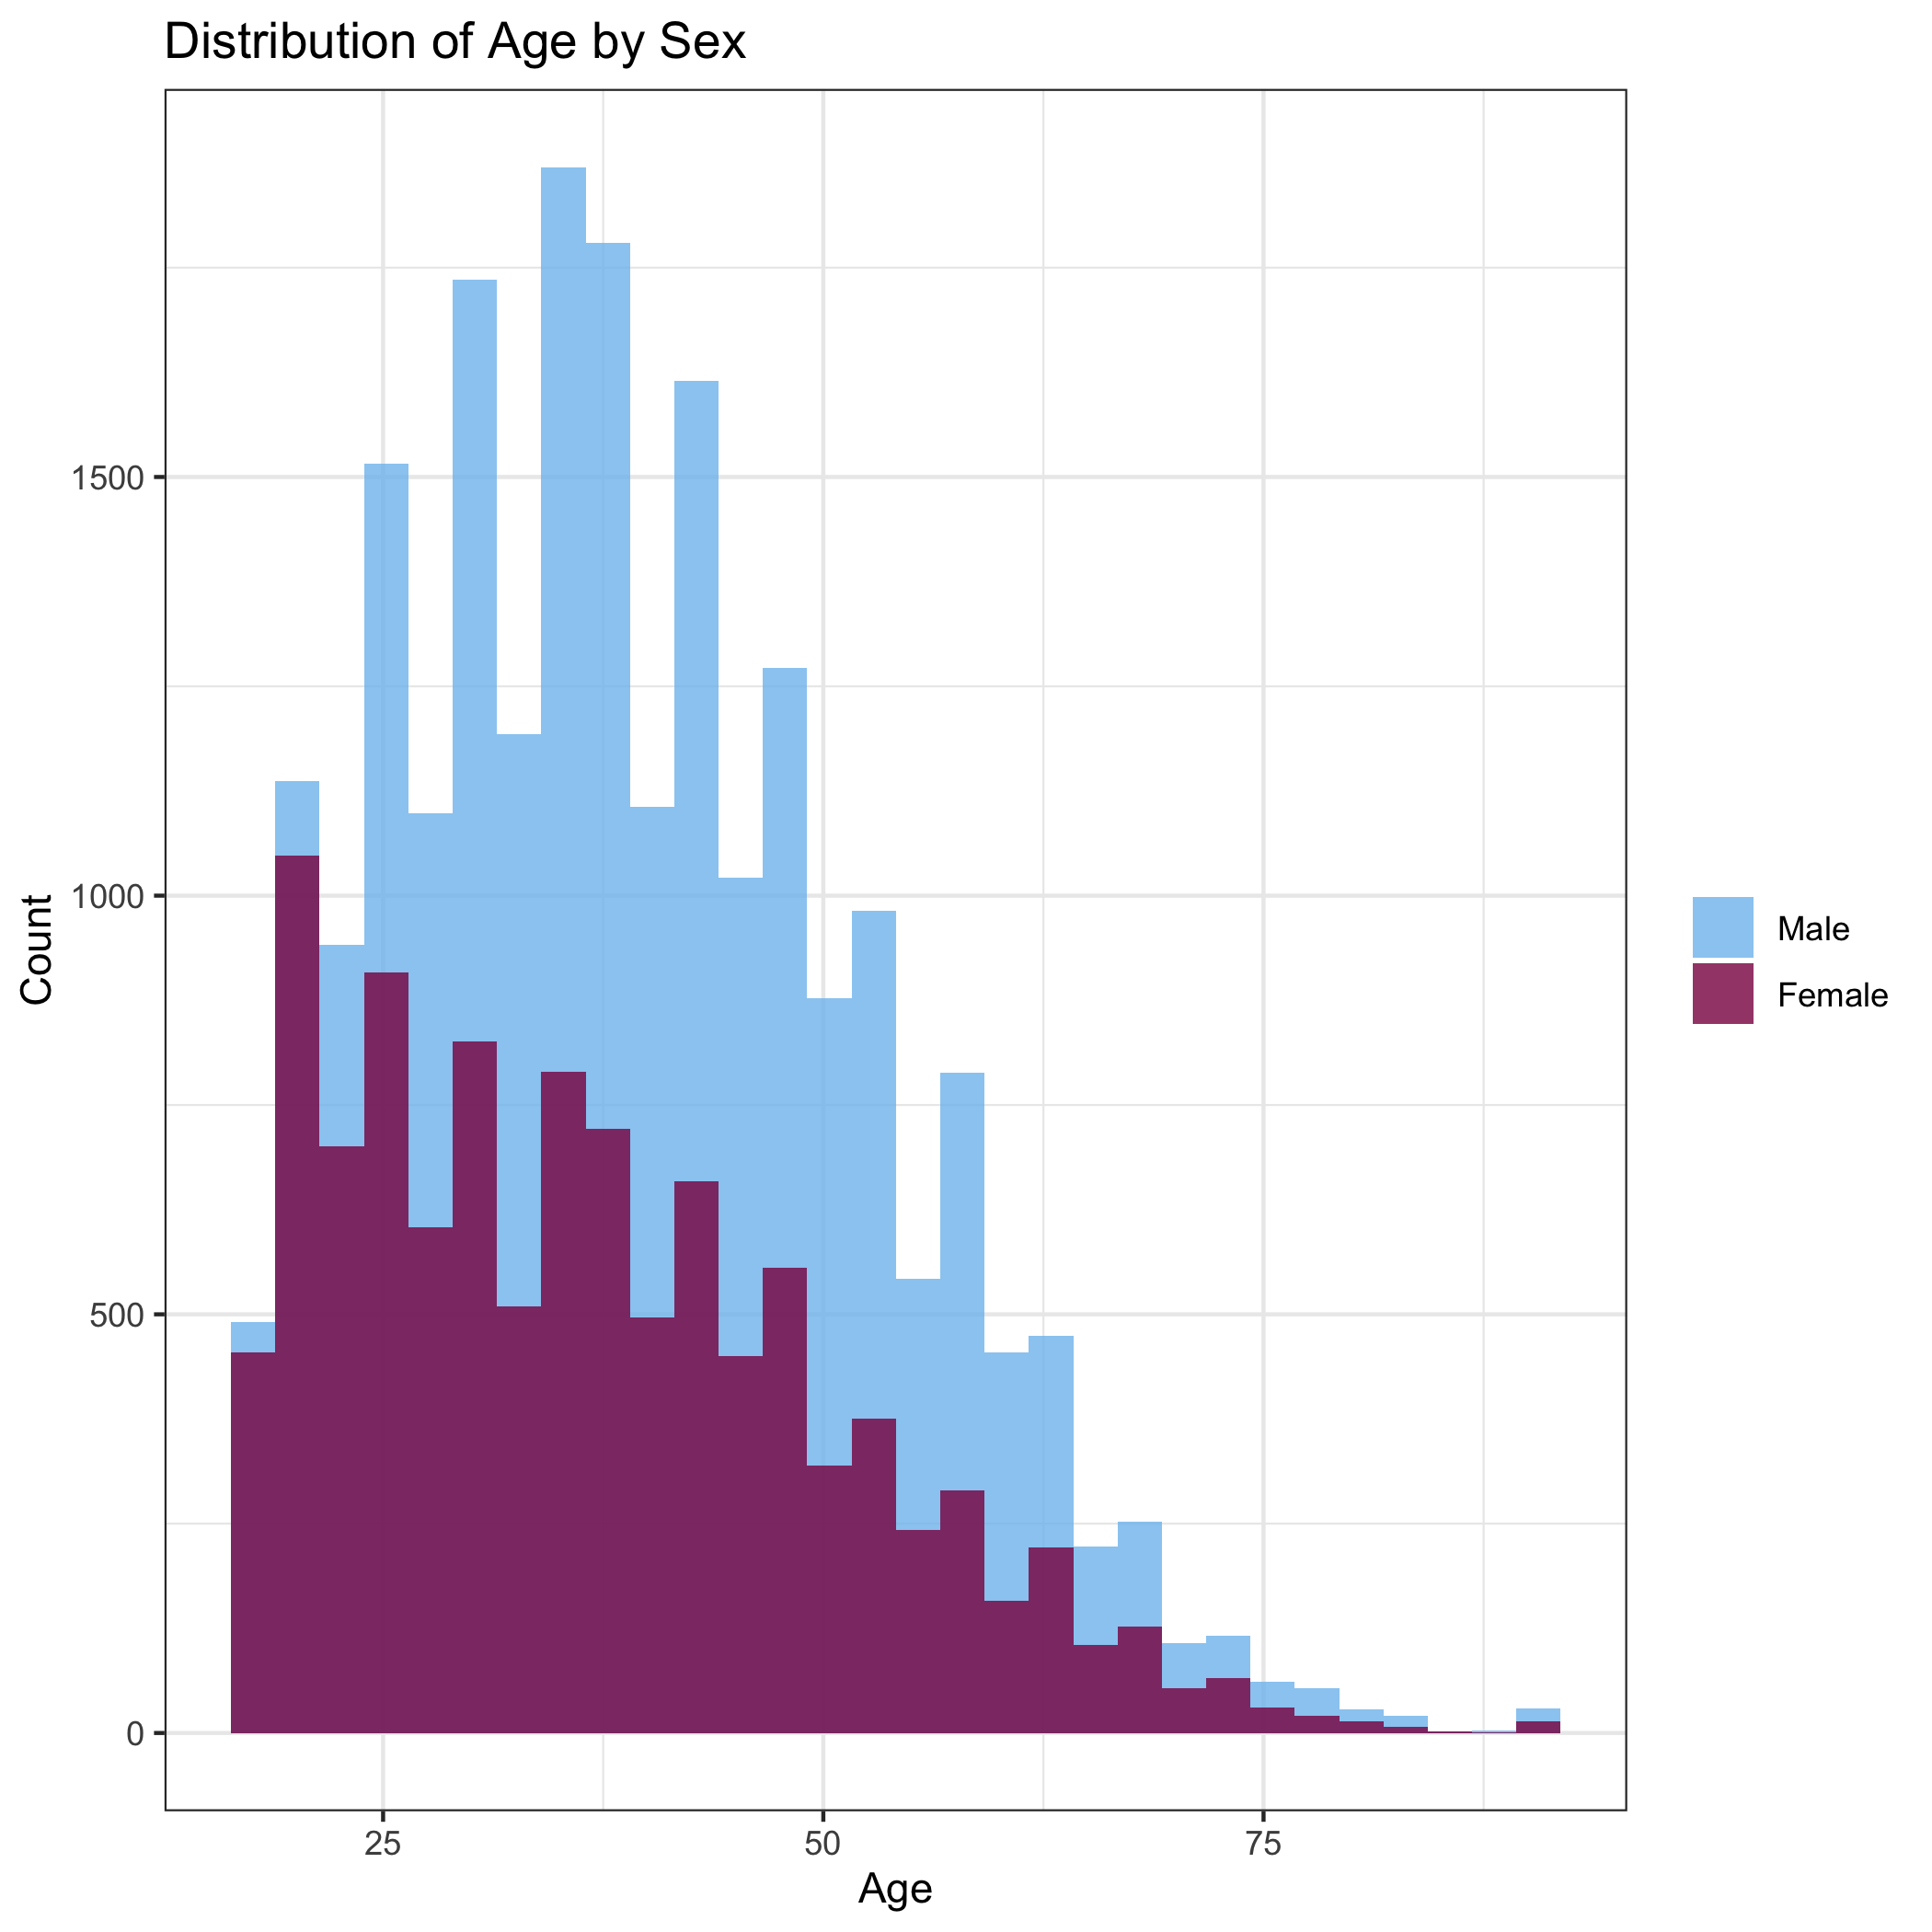
\includegraphics{../images/Plot_1_Distribution_of_Age_by_Sex.png}

\hypertarget{educational-leve-and-income}{%
\paragraph{Educational Leve and
Income}\label{educational-leve-and-income}}

We observe from the following graphs that a majority of individuals
earning greater than \$50,000 a year only accomplished high school
irrespective of sex or ethnical background.

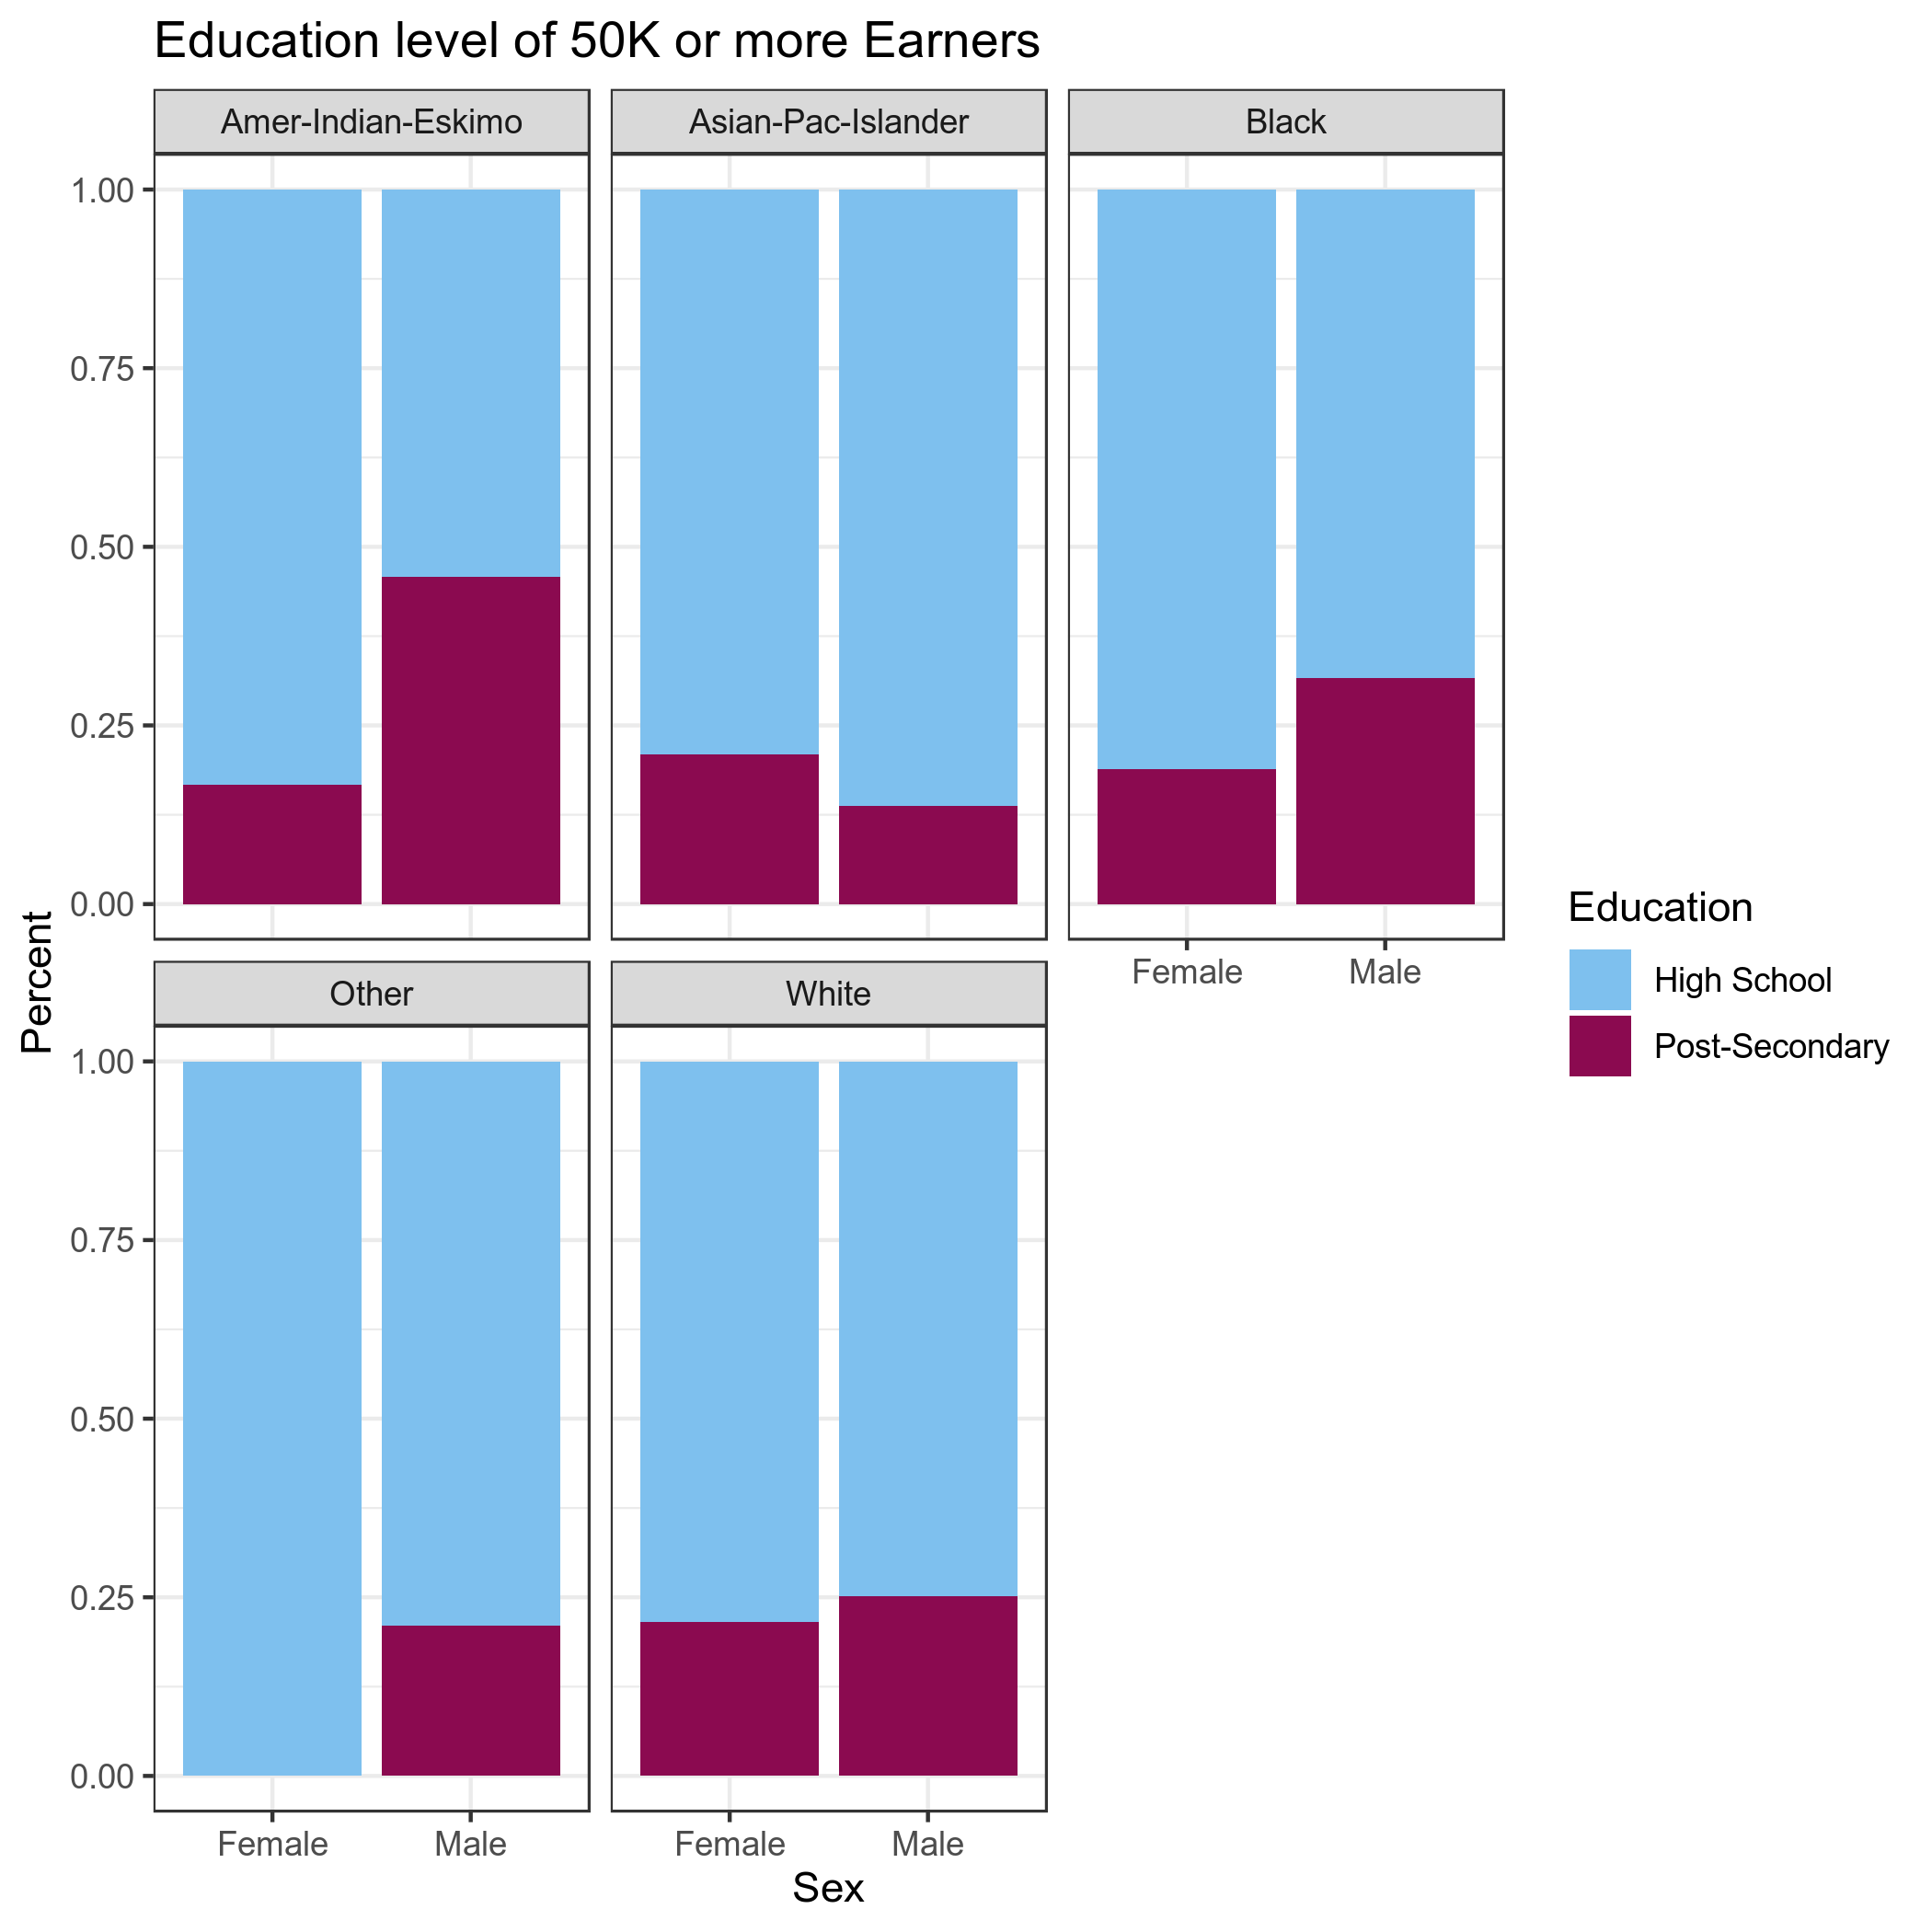
\includegraphics{../images/Plot_2_Education_Level_of_50K_or_more_Earners.png}

\hypertarget{number-of-work-hours-and-age}{%
\paragraph{Number of Work Hours and
Age}\label{number-of-work-hours-and-age}}

We can deduce from the graph below that individuals work the most hours
between their 40's and 60's (probably full time at 40 hours or more a
week) and that employees under 20 and over 80 years of age work the same
number of hours (probably part time at 25 hours)

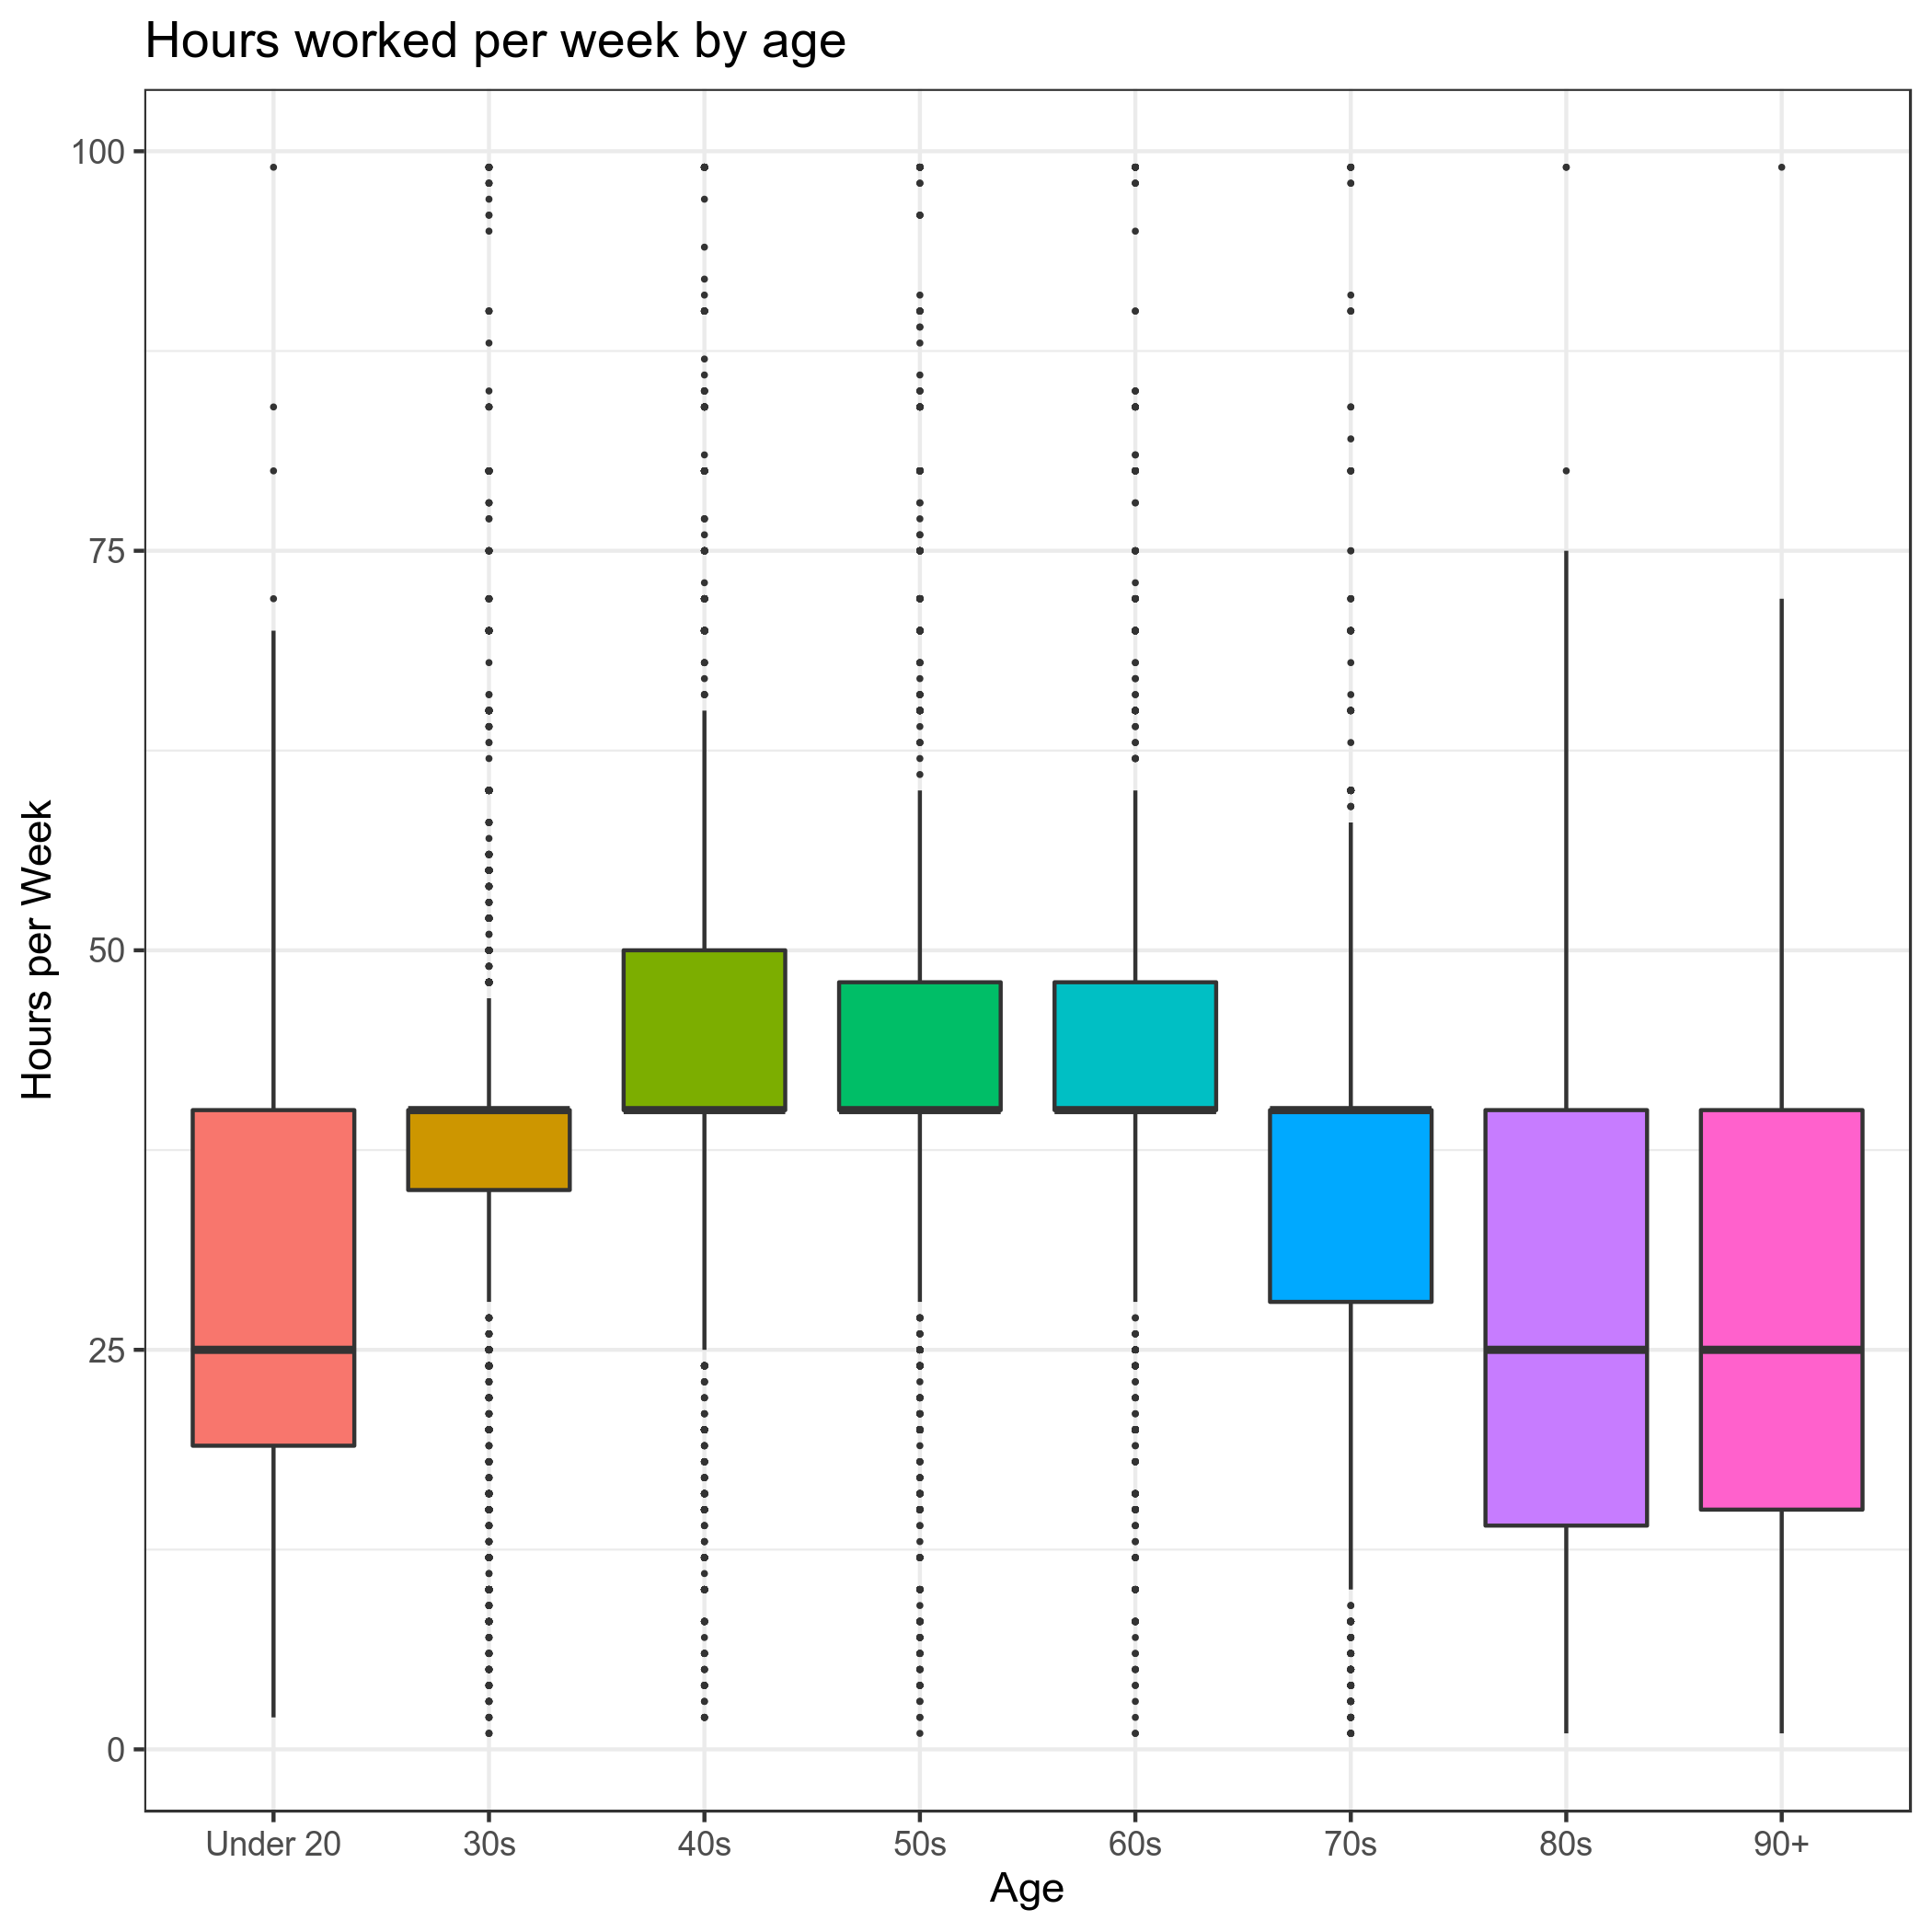
\includegraphics{../images/Plot_3_Hours_worked_per_week_by_age.png}

\hypertarget{marital-status-and-number-of-hours-worked}{%
\paragraph{Marital Status and Number of Hours
Worked}\label{marital-status-and-number-of-hours-worked}}

The plot below shows that the working hours between married individuals
and single employees are similar.

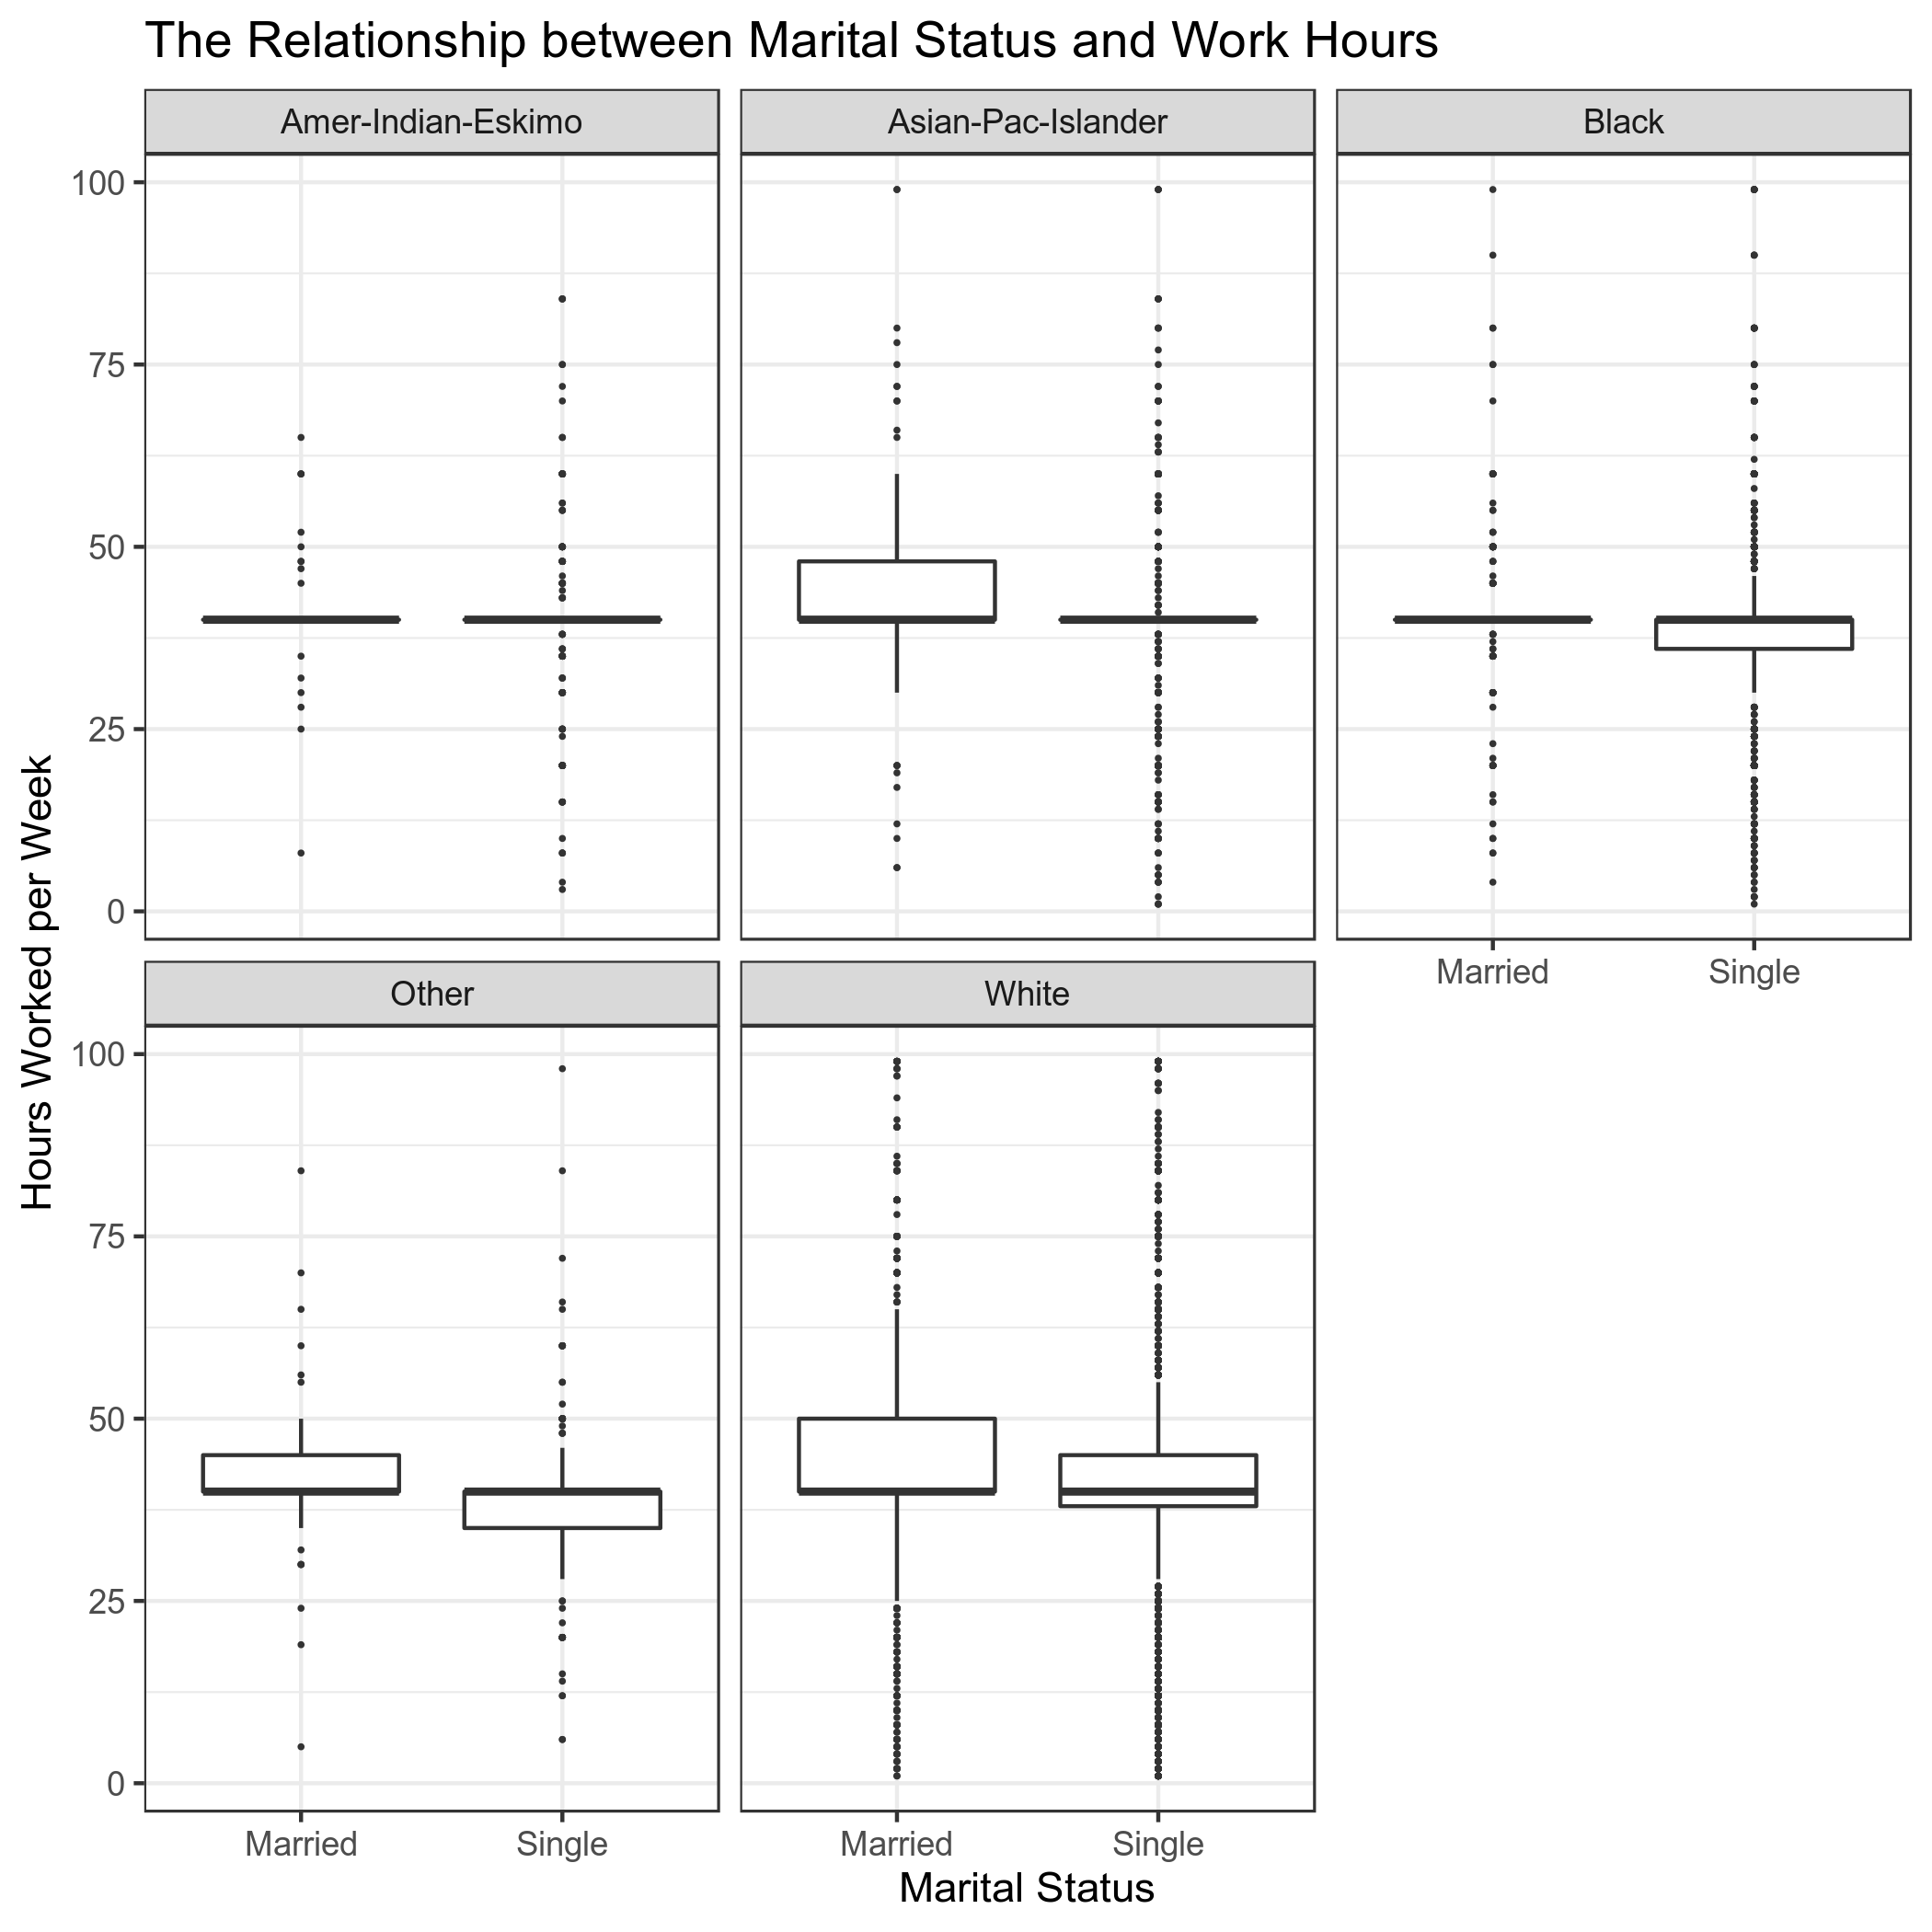
\includegraphics{../images/Plot_4_Marital_Status_and_Work_Hours.png}

\hypertarget{analysis}{%
\subsubsection{Analysis}\label{analysis}}

\begin{enumerate}
\def\labelenumi{\arabic{enumi}.}
\tightlist
\item
  Is earning more than 50K correlated with the education level, marital
  status, and hours worked per week?
\end{enumerate}

Plots showing the relationship between income and each variable
separately. For example, we will perform a logistic regression to show
the the difference between individuals earning more than 50,000 a year
and those who don't using the educational level as the independent
variable.

\textless\textless\textless\textless\textless\textless\textless{} HEAD

\#\texttt{\{r\}\ tidy(readRDS("../data/income\_education.rds"))\ augment(readRDS("../data/income\_education.rds"))\ glance(readRDS("../data/income\_education.rds"))}

=======
\textgreater\textgreater\textgreater\textgreater\textgreater\textgreater\textgreater{}
upstream/master \#```\{r, readRDS for analysis\#2\}
readRDS(``../data/hours\_age.rds'')

readRDS(``../data/hours\_relationship.rds'')

readRDS(``../data/hours\_education.rds'')

readRDS(``../data/hours\_sex.rds'')

\#Relationship of all variables together:
readRDS(``../data/hours\_all.rds'')

```

\hypertarget{results}{%
\subsubsection{Results}\label{results}}

\hypertarget{discussion}{%
\subsubsection{Discussion}\label{discussion}}

\hypertarget{conclusion}{%
\subsubsection{Conclusion}\label{conclusion}}


\end{document}
